\documentclass{article}
\usepackage{tikz}
\begin{document}
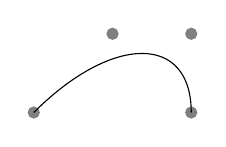
\begin{tikzpicture}
\filldraw[gray] (0,0) circle (2pt)
		        (1,1) circle (2pt)
				(2,1) circle (2pt)
				(2,0) circle (2pt);
	\draw (0,0) .. controls (1,1) and (2, 1) .. (2,0);
\end{tikzpicture}

\begin{tikzpicture}
\draw (-1.5, 0) -- (1.5, 0);
\draw (0, -1.5) -- (0, 1.5);

\draw (-1,0) .. controls(-1, 0.555) and (-0.555,1) .. (0,1)
		     .. controls(0.555, 1) and (1, 0.555) .. (1, 0);
\end{tikzpicture}
\tikz \draw (0,0) circle (10pt);
\tikz \draw (0,0) ellipse (20pt and 10pt);
\begin{tikzpicture}
\tikzstyle help lines=[color=blue!50,very thin]	
\tikzstyle mygrid=[style=help lines,color=blue!50]
...
\draw[style=mygrid] (0,0) grid (5,5);
%\tikzstyle help lines=[color=blue!50,very thin]
%\tikzstyle Karl’s grid=[style=help lines,color=blue!50]
%...
%\draw[style=Karl’s grid] (0,0) grid (5,5);
%\draw[step = .5cm, gray, very thin] (-1.4, -1.4) grid (1.4, 1.4);
\draw (-1.5, 0) -- (1.5, 0);
\draw (0, -1.5) -- (0, 1.5);
\draw (0, 0) circle (1cm);
%\draw (-0.5, -0.5) rectangle (-1,-1);
\end{tikzpicture}
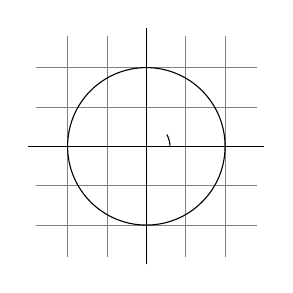
\begin{tikzpicture}%[scale=3]
\draw[step=.5cm,gray,very thin](-1.4,-1.4) grid (1.4,1.4);
\draw (-1.5,0) -- (1.5,0);
\draw (0,-1.5) -- (0,1.5);
\draw (0,0) circle (1cm);
\draw (3mm, 0mm) arc (0:30:3mm);
\end{tikzpicture}
\begin{tikzpicture}
 \draw (0,0) -- (0,1);
 \draw (0,2) arc (0:315:1.75cm and 1cm);
\end{tikzpicture}
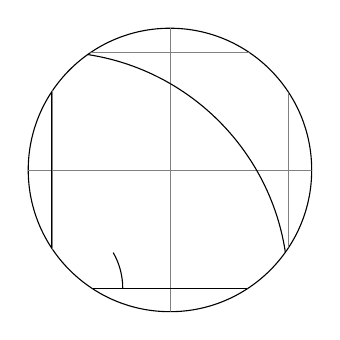
\begin{tikzpicture}[scale=3]
\clip[draw] (0.5,0.5) circle (.6cm);
\draw[step=.5cm,gray,very thin] (-1.4,-1.4) grid (1.4,1.4);
\draw (-1.5,0) -- (1.5,0);
\draw (0,-1.5) --  (0,1.5);
\draw (0,0) circle (1cm);
\draw (3mm,0mm) arc (0:30:3mm);
\end{tikzpicture}
\tikz \draw[x=1.57ex,y=1ex] %(0,0) sin (1,1) cos (2,0) sin (3,-1) cos (4,0)
							(0,1) cos (1,0) sin (2,-1) cos (3,0) sin(4,1);
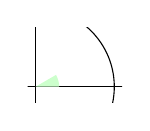
\begin{tikzpicture}
\clip (-0.1,-0.2) rectangle (1.1, 0.75);
\draw[step=.5cm,gray,very thin] (-1.4,1.4) grid (1.4,1.4);
\draw (-1.5,0) -- (1.5,0);
\draw (0,-1.5) -- (0,1.5);
\draw (0,0) circle (1cm);
\fill[green!20!white] (0,0) -- (3mm,0mm) arc(0:30:3mm) -- (0,0);
\end{tikzpicture}
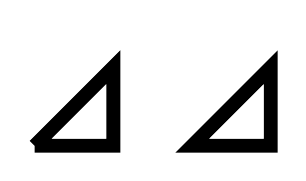
\begin{tikzpicture}[line width=5pt]
\draw (0,0) -- (1,0) -- (1,1) -- (0,0);
\draw (2,0) -- (3,0) -- (3,1) -- cycle;
\useasboundingbox (0,1.5);
\end{tikzpicture}
\tikz \shade (0,0) rectangle (2,1) (3,0.5) circle (.5cm);
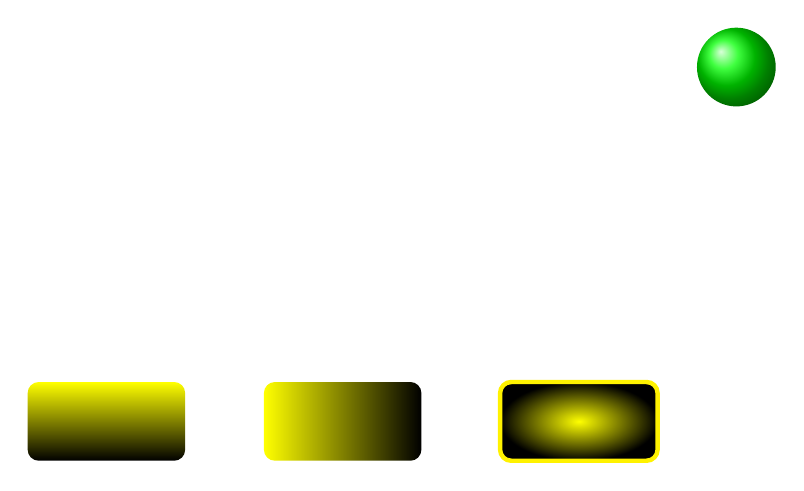
\begin{tikzpicture}[rounded corners, ultra thick]
\shade[top color=yellow,bottom color=black] (0,0) rectangle +(2,1);
\shade[left color=yellow,right color = black] (3,0) rectangle +(2,1);
\shade[inner color=yellow, outer color=black, draw=yellow] (6,0) rectangle +(2,1);
\shade[ball color=green] (9,5) circle (.5cm);
\end{tikzpicture}

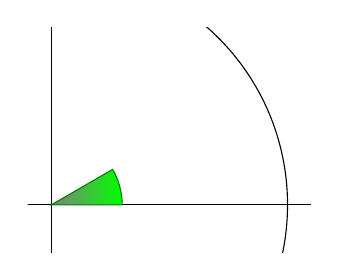
\begin{tikzpicture}[scale=3]
\clip (-0.1,-0.2) rectangle (1.1,0.75);
\draw[step=.5cm,very thin] (1.4,1.4) grid (1.4,1.4);
\draw (-1.5,0) -- (1.5,0);
\draw (0,-1.5) -- (0,1.5);
\draw (0,0) circle (1cm);
\shadedraw[left color=gray,right color=green,draw=green!50!black]
(0,0) -- (3mm,0mm) arc (0:30:3mm) -- cycle;
\end{tikzpicture}
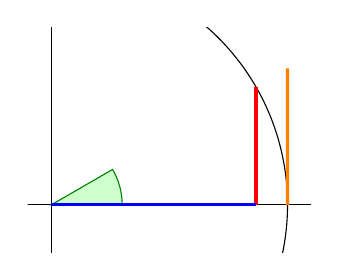
\begin{tikzpicture}[scale=3]
\clip (-0.1,-0.2) rectangle (1.1,0.75);
\draw[step=.5cm,very thin] (1.4,1.4) grid (1.4,1.4);
\draw (-1.5,0) -- (1.5,0);
\draw (0,-1.5) -- (0,1.5);
\draw (0,0) circle (1cm);
\filldraw[fill=green!20,draw=green!50!black]
(0,0) -- (3mm,0mm) arc (0:30:3mm) -- cycle;
\draw[red,very thick] (30:1cm) -- +(0,-0.5);
\draw[blue, very thick] (30:1cm) ++(0,-0.5) -- (0,0);
\draw[orange, very thick] (1,0) -- (intersection of 1,0--1,1 and 0,0--30:1cm);
\end{tikzpicture}
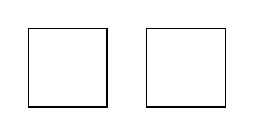
\begin{tikzpicture}
\def\rectanglepath{-- ++(1cm,0cm) -- ++(0cm,1cm) -- ++(-1cm,0cm) -- cycle}
\draw (0,0) \rectanglepath;
\draw (1.5,0) \rectanglepath;
\end{tikzpicture}
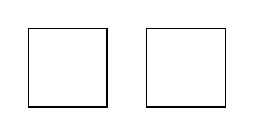
\begin{tikzpicture}
\def\rectanglepath{-- +(1cm,0cm) -- +(1cm,1cm) -- +(0cm,1cm) -- cycle}
\draw (0,0) \rectanglepath;
\draw (1.5,0) \rectanglepath;
\end{tikzpicture}
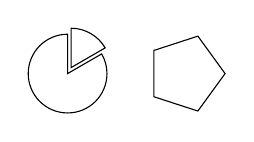
\begin{tikzpicture}[scale=0.5]
\draw (0,0) -- (90:1cm) arc (90:360:1cm) arc (0:30:1cm) -- cycle;
\draw (60:5pt) -- +(30:1cm) arc (30:90:1cm) -- cycle;
\draw (3,0) +(0:1cm) -- +(72:1cm) -- +(144:1cm) -- +(216:1cm) -- +(288:1cm)
		-- cycle;
\end{tikzpicture}
\begin{tikzpicture}[ultra thick]
\draw (0,0) -- (0,1);
\begin{scope}[thin]
\draw (1,0) -- (1,1);
\draw (2,0) -- (2,1);
\end{scope}
\draw (3,0) -- (3,1);
\end{tikzpicture}

\begin{tikzpicture}[even odd rule, rounded corners = 2pt, x = 10pt, y = 10pt]
\filldraw[fill= orange] (0,0) rectangle (1,1)
		[xshift=5pt,yshift=5pt] (0,0) rectangle (1,1)
		[rotate=30] (-1,-1) rectangle (2,2);
\end{tikzpicture}
\end{document}
